\chapter{Potential Fitting}







%%%%%%%%%%%%%%%%%%%%%%%%%%%%%%%%%%%%%%%%%%%%%%%%%%%%%%%%%%%%%%%%%%%%%%%%%%%%%%%%%%%%%%%%%%%%%%%%%%%%%%%%%%
%  Iron FCT
%
%%%%%%%%%%%%%%%%%%%%%%%%%%%%%%%%%%%%%%%%%%%%%%%%%%%%%%%%%%%%%%%%%%%%%%%%%%%%%%%%%%%%%%%%%%%%%%%%%%%%%%%%%%

\section{Iron EAM Potential (FCT)}

The final Iron potential consists of 3 functions.

\begin{list}
\item Fe-Fe Pair
\item Fe Density
\item Fe Embedding
\end{list}



\subsection{Input File}

\begin{lstlisting}[style=sPseudo,caption={Iron potential input file for fitting.}]
# Run types:   plot, e, ef, efs, bp, es, rss, fit
run type=fit

#
wd option=1

# Memory
mem bp=2GB efs=2GB

# Random settings
random seed=100

# Display
display output=1

# Input files/dirs
potential dir="pot/fe" index_file="fe.pot" embedding_range_factor=1.5
configs dir="configs"
bp dir='bp' bp_file='bp.dat' eos_size=6 eos_strain=0.01 ec_size=6 ec_strain=0.01

# Rss weights
# config * (e + f + s)   bp * (a0 + e0 + b0 + ec + g + e + v)
# Weighting config = 0 and bp = 0 should turn off those calcs
rss_weights config=0.0001 energy=20.0 force=1.0 stress=1.0 bp=100.0 a0=5.0 e0=5.0 b0=1.0 ec=1.0 g=1.00 e=1.00 v=1.00 negec=1000.0

# Rss weights - max density, outside of accepted range
rss_max_density min=0.1 max=100.0 scale_factor=10.0 scale_exponent=4.0 zero_density_factor=1.0e8

# Fitting options
fitting top_parameters=100 load_top_parameters=0 oversized_parameters=2.0,0.25,0.5,0.5,0.5

fit1 type=random random_size=5000 oversized_parameters=True
fit2 type=random random_size=5000 oversized_parameters=False
fit3 type=ga gens=10 pop_size=1000 fresh_size=250 no_clone_var=0.001 gen_variation_multiplier=0.2
fit4 type=sa sa_temp_start=10.0 sa_temp_end=0.01 sa_loops_t=20 sa_loops_i=1000 sa_step=0.1 sa_step_factor=0.25 oversized_parameters=True
fit5 type=ga gens=10 pop_size=1000 fresh_size=250 no_clone_var=0.001 gen_variation_multiplier=0.2
fit6 type=sa sa_temp_start=10.0 sa_temp_end=0.01 sa_loops_t=12 sa_loops_i=1000 sa_step=0.1 sa_step_factor=0.25 oversized_parameters=False

# Fit Results
fit_results results_dir=results

# DFT
dft Al=32,-1264.06398979,Ry,-3.36,eV Fe=16,-5268.188,Ry,-4.316,eV Pd=32,-16384.958,Ry,-3.91,eV
\end{lstlisting}




\subsection{Bulk Properties File}

\begin{lstlisting}[style=sPseudo,caption={Bulk properties file for fitting.}]
# Bulk Properties File
units pressure=GPA length=ang energy=ev

# ORTHORHOMBIC  C11 C22 C33 C44 C55 C66 C12 C13 C23  
FEFCC1 potlabel=FE b0=222 alat=3.59 uv=0.96,1.00,.96 e0=-4.27 ec=365.6,298.7,364.6,186.3,266.8,186.3,141.6,233.8,130.4 type=fcc expansion=4 rcut=6.5 amu_per_crystal=224.00


#FEFCC1 potlabel=FE b0=222 alat=3.59 uv=0.952,1.0,0.952 e0=-4.27 ec=365.6,298.7,364.6,186.3,266.8,186.3,141.6,233.8,130.4 type=fcc expansion=4 rcut=6.5 amu_per_crystal=224.00
# CUBIC  C11 C12 C44  
#FEFCC1 potlabel=FE b0=222 alat=3.59 uv=0.952,1.0,0.95 e0=-4.27 ec=343.6,168.7,213.0 type=fcc expansion=4 rcut=6.5 amu_per_crystal=224.00
#FEFCC1 potlabel=FE b0=222 alat=3.42 uv=1.0 e0=-4.27 ec=365,137,186 type=fcc expansion=4 rcut=6.5 amu_per_crystal=224.00
\end{figure}


\subsection{Potential Files}

\begin{lstlisting}[style=sPseudo,caption={Main index file: fe.pot}]
POTNAME fe_pot

START
F_ON true
FILE fe_pair.pot
LABEL FE FE
F_TYPE PAIR
END

START
F_ON true
FILE fe_dens.pot
LABEL FE
F_TYPE DENS
F_GROUP Group1
END

START
F_ON true
FILE fe_embe.pot
LABEL FE
F_TYPE EMBE
F_GROUP Group1
END
\end{lstlisting}

\begin{lstlisting}[style=sPseudo,caption={Pair function: fe\_pair.pot}]
#TYPE cubic_spline_zbl
#P -36.5540536943 21.8144454622 -1.06882955227 2.17017966425 6.69737742394 2.58940859512 8.29763238337 -0.556459419716 -5.65030529508 3.78427535852 0.264082774201 0.062236557983 -0.00344996782068 -0.180560254415 0.124961363986 -0.0322144195924 0.000541478517592 0.0 
#PF 1.8 2.0 2.1 2.2 2.3 2.4 2.5 2.6 2.7 2.8 3.0 3.3 3.7 4.2 4.7 5.3 6.0 6.5 26.0 26.0 1.2 1.8 1.0 
#VR 2.0
\end{lstlisting}

\begin{lstlisting}[style=sPseudo,caption={Density function: fe\_dens.pot}]
#TYPE cubic_knot_spline_fixed_end
#P -1.94938564301 30.3556213379 24.3362083435 34.9576034546 16.2302913666 17.857875824 7.66438293457 1.23997938633 0.442521393299 0.109044238925 0.0200536046177 0.00229621282779 0.00255827326328 0.00108765787445 7.98819164629e-05 4.18824820372e-05 4.40689618699e-05 
#PF 0.0 0.0194847 0.0454644 0.0974237 0.227322 0.37021 0.688461 1.00671 1.32496 1.64321 1.96146 2.27972 2.59797 2.91622 3.23447 3.55272 3.87097 5.0 0.0 0.0 
#VR 0.0
\end{lstlisting}

\begin{lstlisting}[style=sPseudo,caption={Embedding functional: fe\_embe.pot}]
#TYPE ackland_embedding
#P -17.5580856865 0.544337185381 1.0 
#PF 0.0 
#VR 0.0
\end{lstlisting}



\FloatBarrier
\subsection{Function Plots}

\begin{figure}[ht] 
  \begin{minipage}[b]{0.5\linewidth}
    \centering
    \includegraphics[width=.9\linewidth]{chapters/results_potential_fitting/iron-fct/fe_pair.eps} 
    \caption{Fe-Fe Pair Function} 

  \end{minipage}%%
  \begin{minipage}[b]{0.5\linewidth}
    \centering
    \includegraphics[width=.9\linewidth]{chapters/results_potential_fitting/iron-fct/fe_pair_zoom.eps} 
    \caption{Fe-Fe Pair Function (zoom)} 
  \end{minipage} 
  \begin{minipage}[b]{0.5\linewidth}
    \centering
    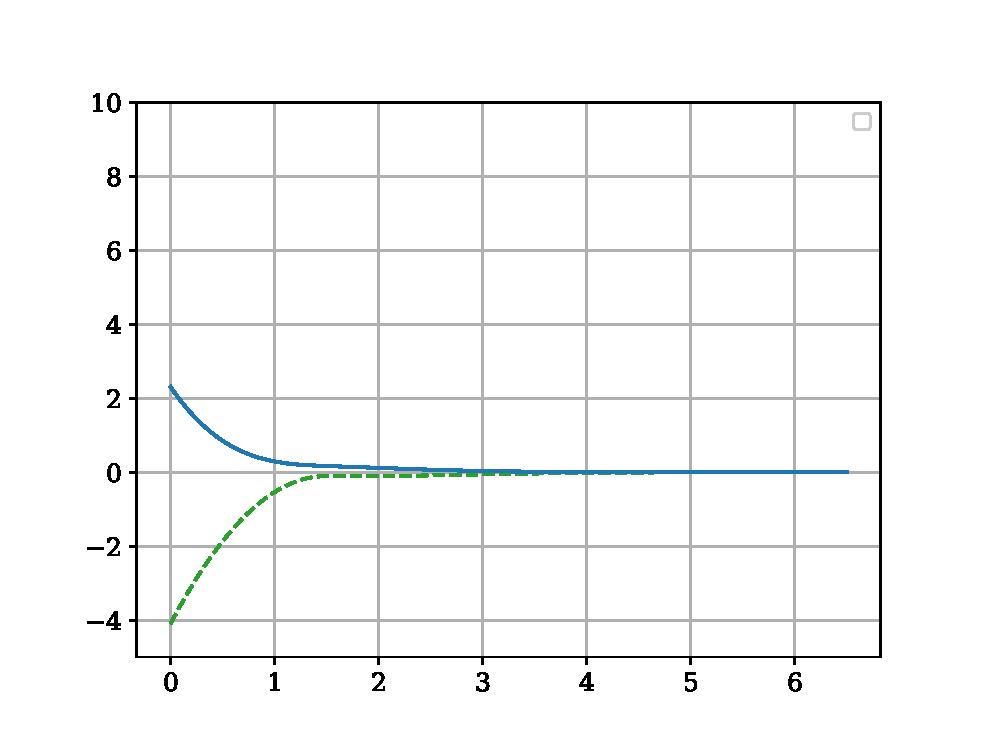
\includegraphics[width=.9\linewidth]{chapters/results_potential_fitting/iron-fct/fe_dens.eps} 
    \caption{Fe Density Function} 
  \end{minipage}%% 
  \begin{minipage}[b]{0.5\linewidth}
    \centering
    \includegraphics[width=.9\linewidth]{chapters/results_potential_fitting/iron-fct/fe_embe.eps} 
    \caption{Fe Embedding Function} 
  \end{minipage} 
  \label{fig:ironPotentialPlots} 
\end{figure}


\FloatBarrier
\subsection{Properties Calculated from Potential}


\begin{lstlisting}[style=sPseudo,caption={Potential Properties}]
========================================================================================
========================================================================================
BP  0
========================================================================================
========================================================================================
a0                  3.590000      3.484442      0.011143
v0                               10.576441
e0                 -4.270000     -4.268041      0.000004
b0                  1.385502      1.551103      0.027424

Calculated Stiffness Matrix (GPA)
    326.508178    144.251699    254.248660      0.000000      0.000000      0.000000
    144.251699    325.505659    151.099600      0.000000      0.000000      0.000000
    254.248660    151.099600    326.508178      0.000000      0.000000      0.000000
      0.000000      0.000000      0.000000    166.136047      0.000000      0.000000
      0.000000      0.000000      0.000000      0.000000    267.522174      0.000000
      0.000000      0.000000      0.000000      0.000000      0.000000    166.136047
Known Stiffness Matrix (GPA)
    365.600000    141.600000    233.800000      0.000000      0.000000      0.000000
    141.600000    298.700000    130.400000      0.000000      0.000000      0.000000
    233.800000    130.400000    364.600000      0.000000      0.000000      0.000000
      0.000000      0.000000      0.000000    186.300000      0.000000      0.000000
      0.000000      0.000000      0.000000      0.000000    266.800000      0.000000
      0.000000      0.000000      0.000000      0.000000      0.000000    186.300000

Other calculated properties
===========================
Bulk Modulus B0 (Reuss):             1.415347    (    226.782064) GPA
Bulk Modulus B0 (Voigt):             1.440785    (    230.857992) GPA
Tetragonal Shear:                    0.568731    (      0.568731) GPA
Shear Modulus G:                     1.036855    (    166.136047) GPA
Shear Modulus G (Reuss):             0.588484    (     94.293259) GPA
Shear Modulus G (Voigt):             0.927123    (    148.553657) GPA
Young's Modulus E:                   1.931722    (    309.521186) GPA
Poisson Ratio                        0.643907
Cachy Pressure:                     -0.136580    (    -21.884349) GPA
Melting Point:                    4242.440618K
Cubic Stability:                     1.000000 (1=Stable, 0=Unstable)
Stability:                           1.000000 (1=Stable, 0=Unstable)
\end{lstlisting}




\FloatBarrier
\subsection{Function Plots}

\begin{figure}[ht] 
  \begin{minipage}[b]{0.5\linewidth}
    \centering
    \includegraphics[width=.9\linewidth]{chapters/results_potential_fitting/iron-fcc-eos-ec/eos_0.eps} 
    \caption{Fe-Fe Pair Function} 
  \end{minipage}
  \begin{minipage}[b]{0.5\linewidth}
    \centering
    \includegraphics[width=.9\linewidth]{chapters/results_potential_fitting/iron-fcc-eos-ec/ec_0.eps} 
    \caption{Fe-Fe Pair Function (zoom)} 
  \end{minipage} 
  \label{fig:ironPotentialPlots} 
\end{figure}


\FloatBarrier










\section{Palladium EAM Potential}


\subsection{Input File}

\begin{lstlisting}[style=sPseudo,caption={Palladium potential input file for fitting.}]
\end{lstlisting}



\subsection{Bulk Properties File}

\begin{lstlisting}[style=sPseudo,caption={Bulk properties file for fitting.}]
\end{lstlisting}

\subsection{Potential Files}

\begin{lstlisting}[style=sPseudo,caption={Main index file: pd.pot}]
\end{lstlisting}

\begin{lstlisting}[style=sPseudo,caption={Pair function: pd\_pair.pot}]
\end{lstlisting}

\begin{lstlisting}[style=sPseudo,caption={Pair function: pd\_dens.pot}]
\end{lstlisting}

\begin{lstlisting}[style=sPseudo,caption={Pair function: pd\_embe.pot}]
\end{lstlisting}



\FloatBarrier
\subsection{Function Plots}





\FloatBarrier
\subsection{Properties Calculated from Potential}


\begin{lstlisting}[style=sPseudo,caption={Potential Properties}]
\end{lstlisting}










\subsection{Potential Function Files}

The final Iron-Palladium potential consists of 7 functions.

\begin{list}
\item Fe-Fe Pair
\item Fe-Pd Pair
\item Pd-Pd Pair
\item Fe Density
\item Pd Density
\item Fe Embedding
\item Pd Embedding
\end{list}

\begin{lstlisting}[style=sFortran,caption={Potential}]
POTNAME fepd_pot

!###########################
!# PAIR
!###########################

! Pair FE FE
START
FILE              fe_pair_analytic.pot
FIT               fe_pair.fit
LABEL             FE   FE
F_ON true
F_TYPE            PAIR            ! PAIR DENS EMBE
F_GROUP
R_CUT              6.5
ZOOR     true  ! zero out of range
END

! Pair FE PD
START
FILE              fepd_pair_analytic.pot
FIT               fepd_pair.fit
LABEL             FE   PD
F_ON true
F_TYPE            PAIR            ! PAIR DENS EMBE
F_GROUP
R_CUT              6.5
ZOOR     true  ! zero out of range
END

! Pair PD PD
START
FILE              pd_pair_analytic.pot
FIT               pd_pair.fit
LABEL             PD   PD
F_ON true
F_TYPE            PAIR            ! PAIR DENS EMBE
F_GROUP
R_CUT              6.5
ZOOR     true  ! zero out of range
END


!###########################
!# DENSITY
!###########################

! FE Density
START
FILE              fe_dens_analytic.pot
FIT               fe_dens.fit
LABEL             FE
F_ON true
F_TYPE            DENS            ! PAIR DENS EMBE
F_GROUP           1
R_CUT             6.5
END

! PD Density
START
FILE              pd_dens_analytic.pot
FIT               pd_dens.fit
LABEL             PD
F_ON true
F_TYPE            DENS            ! PAIR DENS EMBE
F_GROUP           1
R_CUT             6.5
END


!###########################
!# EMBEDDING
!###########################

! FE Embedding
START
FILE              fe_embe_analytic.pot
FIT               fe_embe.fit
LABEL             FE
F_ON true
F_TYPE            EMBE            ! PAIR DENS EMBE
F_GROUP           1
R_CUT              6.5
ZOOR     true  ! zero out of range
END

! PD Embedding
START
FILE              pd_embe_analytic.pot
FIT               pd_embe.fit
LABEL             PD
F_ON true
F_TYPE            EMBE            ! PAIR DENS EMBE
F_GROUP           1
R_CUT              6.5
ZOOR     true  ! zero out of range
END
\end{lstlisting}





\begin{lstlisting}[style=sFortran,caption={Potential}]
#FIT A
#PS  -1.54763217114 -3.84020969698 -0.164438468948 0.0899525241411 -0.0968867227903 0.0478808975252 0.0510228350092 0.0281999363282 -0.0551143973539 -0.124408628134 -0.161531727893 -0.211461860015 -0.0580325839633
#PL  -3.04763217114 -6.84020969698 -3.16443846895 -2.91004747586 -3.09688672279 -0.952119102473 -0.948977164986 -0.971800063671 -1.05511439735 -1.12440862813 -1.16153172789 -1.21146186002 -1.05803258396
#PU  -0.0476321711446 -0.840209696981 2.83556153105 3.08995252414 2.90311327721 1.04788089752 1.051022835 1.02819993633 0.944885602646 0.875591371867 0.838468272103 0.788538139989 0.941967416035
\end{lstlisting}























